
\chapter{Novel Approach: Reprojection
Mapping}\label{novel-approach-reprojection-mapping}

\section{Idea}\label{idea}

A radar range reading reveals the distance to detected targets, but not what angle they are seen under. As explained in \cref{scanning-radar}, this can be solved by scanning the radar antenna to exploit beam directionality. There are however some drawbacks to scanned radars. The increased design complexity and cost of electronic scanning with phased arrays makes a sensor design more expensive. Passive phased arrays have a limited field of view. The motorized parts of mechanical scanning and active phased arrays not only increase cost compared to scanless antennas, but also introduce additional points of failure, higher maintenance requirements and increased power consumption.

This thesis proposes the reprojection method, with which a radar target's source can be determined without the need to scan the sensor. While the target distance is of course already available in the radar range data the target angle must be known in order to build or update a map of the environment. Under certain circumstances the target angle can be extracted from range readings with the reprojection method.

The method requires that the sensor moves at a known speed \(v_R\) through an otherwise static environment. Through the sensor's motion the distance to visible targets will then change over time, which causes a Doppler effect for the entire visible scene. Based on the deviation of a target's measured Doppler speed \(v_D\) from the known sensor movement speed \(v_R\) the magnitude of the angle between the movement vector and the line-of-sight to the same target can then be calculated.

\section{Geometry for the Side-Facing 2D Case}\label{geometry-for-the-side-facing-case}

Assume that the sensor's antenna is sensitive only to co-planar targets --- this can be achieved with antennas that feature a fan-shaped beam pattern that has high sensitivity only around zero elevation. In the simplest case, the antenna is also sensitive only to targets on one side of the path of motion described by the sensor. \Cref{fig:geometry-side} depicts a robot (gray circle) with a radar sensor (triangle) moving at speed $v_R$. The three targets A, B, and C (colored circles) are detected. Targets A and C represent the edge cases: The radar is moving straight towards target A (i.e. $\alpha=0$) and measures its Doppler speed as
\begin{equation} \label{eq:geometry_side_A}
    v_D = v_R\text{, for }\alpha=0.
\end{equation}
At the same time it just passes target C at the point of closest approach with $\alpha=\frac{\pi}{2}$. Target C's Doppler speed will be measured as
\begin{equation} \label{eq:geometry_side_C}
    v_D = 0\text{, for }\alpha=\frac{\pi}{2}.
\end{equation}
Target B finally shows the relationship of $v_D$, $v_R$ and $\alpha$ for all targets on one side of the radar's path, including the extremes in \cref{eq:geometry_side_A,eq:geometry_side_C}:
\begin{equation} \label{eq:geometry_side_B}
    v_D = v_R~\cos(\alpha)\text{, for }0 \leq \alpha \leq \pi
\end{equation}
This is of course also true for already passed targets, which will yield a negative Doppler speed $v_D < 0$. Simply rearranging \cref{eq:geometry_side_B} for $\alpha$ then gives the target's \textit{reprojection angle}
\begin{equation} \label{eq:geometry_side_alpha}
    \alpha = \arccos\left(\frac{v_D}{v_R}\right).
\end{equation}
Note that \cref{eq:geometry_side_alpha} holds, because the scene must be static and hence $-v_R \leq v_D \leq v_R$.

\section{Geometry for the General 2D Case} \label{geometry-for-the-general-case}

\begin{figure}[htp]
    \centering
    \footnotesize
    \begin{subfigure}[t]{0.475\textwidth}
        \def\svgwidth{\linewidth}
        \input{gfx/diagrams/geometry_side.pdf_tex}
        \caption{Side-facing 2D case}
        \label{fig:geometry-side}
    \end{subfigure}%
    \hfill%
    \begin{subfigure}[t]{0.475\textwidth}
        \def\svgwidth{\linewidth}
        \input{gfx/diagrams/geometry_forward.pdf_tex}
        \caption{Forward-facing / general 2D case}
        \label{fig:geometry-forward}
    \end{subfigure}
    \caption{Reprojection geometries}
\end{figure}

In the planar side-facing case, only the principal value of the inverse cosine in \cref{eq:geometry_side_alpha} is used. However, as soon as the radar antenna features angle sensitivities that allow the detection of targets on both sides of the motion path, there will be an angle ambiguity. This is the case for a sensor that is mounted forward-facing or that can detect targets in a field of view of over 180°. This case is practically very relevant as it is of high importance for an obstacle sensor to be sensitive to obstacles in its path rather than just objects located on the side.

\Cref{fig:geometry-forward} visualizes this geometry: For target A the angle is still clear, because according to \cref{eq:geometry_side_A} $\alpha = 0$. Targets B and C however are located at angles $\alpha$ and $-\alpha$, which according to \cref{eq:geometry_side_B} causes the same Doppler speed. In this case, \cref{eq:geometry_side_alpha} will yield an ambiguous result.

It would be possible to resolve this ambiguity by tracking the targets while changing the robot's movement direction as shown in \cref{fig:geometry-turn}. If the robot's bearing is changed by $\beta$, the targets B and C appear at angles $\alpha+\beta$ and $\alpha-\beta$, respectively. The target whose Doppler speed changes to $v_D = v_R~\cos(\alpha+\beta)$ is the one that the robot turned away from, and vice versa for the other target. The drawback is that newly detected targets can only be mapped after a change of bearing, which means that the robot has to drive in a zig-zag path to properly map its environment.

\begin{figure}
    \centering
    \def\svgwidth{0.5\linewidth}
    \input{gfx/diagrams/geometry_turning.pdf_tex}
    \caption{Ambiguity resolution through target tracking during turns}
    \label{fig:geometry-turn}
\end{figure}

For multistatic radars there is however another solution to resolving the angle ambiguity: Using direction of arrival (DOA) information obtained from inter-antenna phase difference measurements (see \cref{direction-of-arrival}). \Cref{fig:geometry-forward} shows that if the radar is mounted at a straight forward angle, a target's DOA indicates the side it is being passed on. If the radar is not facing straight ahead, the DOA value should be tracked so its gradient can be used instead --- If a target's DOA is gradually shifting towards left (target B in \cref{fig:geometry-forward}), it will pass the radar on the left side. On the other hand, if it is gradually shifting towards right, it will pass on the right side (target C in \cref{fig:geometry-forward}).

\section{Geometry for the General 3D Case}\label{geometry-for-the-3d-case}

The geometry in \cref{geometry-for-the-general-case} can be further generalized in a three dimensional geometry. The 3D case is depicted in \cref{fig:3dcase}. The model makes most sense for a robot that can traverse in all three dimensions, like a plane or drone. Hence the blue line in the figure can be called the sensor's flight path vector. Just like in the 2D case, when a static target is detected at range $R$, its radial speed $v_D$ leads to a reprojection angle $\alpha$. The difference is that the possible target location lies not on two points, but on the green circle with radius $R~\sin(\alpha)$ whose origin lies $R~\cos(\alpha)$ away on the flight path vector.

\begin{figure}[htp]
    \begin{subfigure}[t]{.475\textwidth}
        \centering
        \def\svgwidth{5cm}
        \input{gfx/diagrams/outlook_3d.pdf_tex}
        \caption{A target detected at range \(R\) with a relative Doppler speed corresponding to reprojection angle \(\alpha\) will be on a point on the circle (green) around the flight path (blue).}
        \label{fig:3dcase}
    \end{subfigure}%
    \hfill%
    \begin{subfigure}[t]{.475\textwidth}
        \centering
        \def\svgwidth{5cm}
        \input{gfx/diagrams/outlook_doa.pdf_tex}
        \caption{Non-collinear triple receive antenna arrangement.}
        \label{fig:2ddoa}
    \end{subfigure}
    \caption{3D geometry and ambiguity reduction through 2D-DOA.}
\end{figure}

This makes sense because it shows that the 2D case is a special case of the 3D case, where the possible target locations are reduced from the full circle to the intersection points of the circle and the floor plane on which the robot navigates.

The ambiguity could be reduced through a two-dimensional DOA estimation. This is possible if a sensor has three or more non-collinear receiving antennas. The simplest configuration would be the one shown in \cref{fig:2ddoa}, which allows horizontal DOA estimation from the phase difference between \textit{Rx1} and \textit{Rx2}, and vertical DOA estimation between \textit{Rx1} and \textit{Rx3}. However, DOA measurements can not resolve the target location single point like in the 2D case and it would be necessary to implement the target-tracking-during-change-of-motion-vector approach.

With this geometry, reprojection mapping could be used to build probabilistic 3D occupancy gridmaps like in \cite{Hornung2013}, with vehicles moving in 3D space, like the TUM RCS's Modular Airborne Real-Time Testbed (MART)\footnote{\url{https://www.rcs.ei.tum.de/forschung/mart/}} that was also used in other research and publications \cite{Becker2015}.

\section{Geometry for the General 3D Case with Two Sensors} \label{multisensor}
The ambiguities in \cref{geometry-for-the-3d-case} can also be eliminated by using more than one range sensor. In a 2D environment, this makes it possible to do regular trilateration, so reprojection mapping would not be necessary. In the 3D case however, two sensors would be enough for trilateration to pinpoint a target location --- instead, the target would be localized on the intersection circle of two spheres around the sensors, each with a radius equal to the target range. With the addition of reprojection geometry, for each sensor a cone with an opening angle of twice the reprojection angle can be added. The cone's base edge lies on the sphere. A target's location is now known to be at the intersection of the two cones, which is a single point.

\begin{figure}
    \centering
    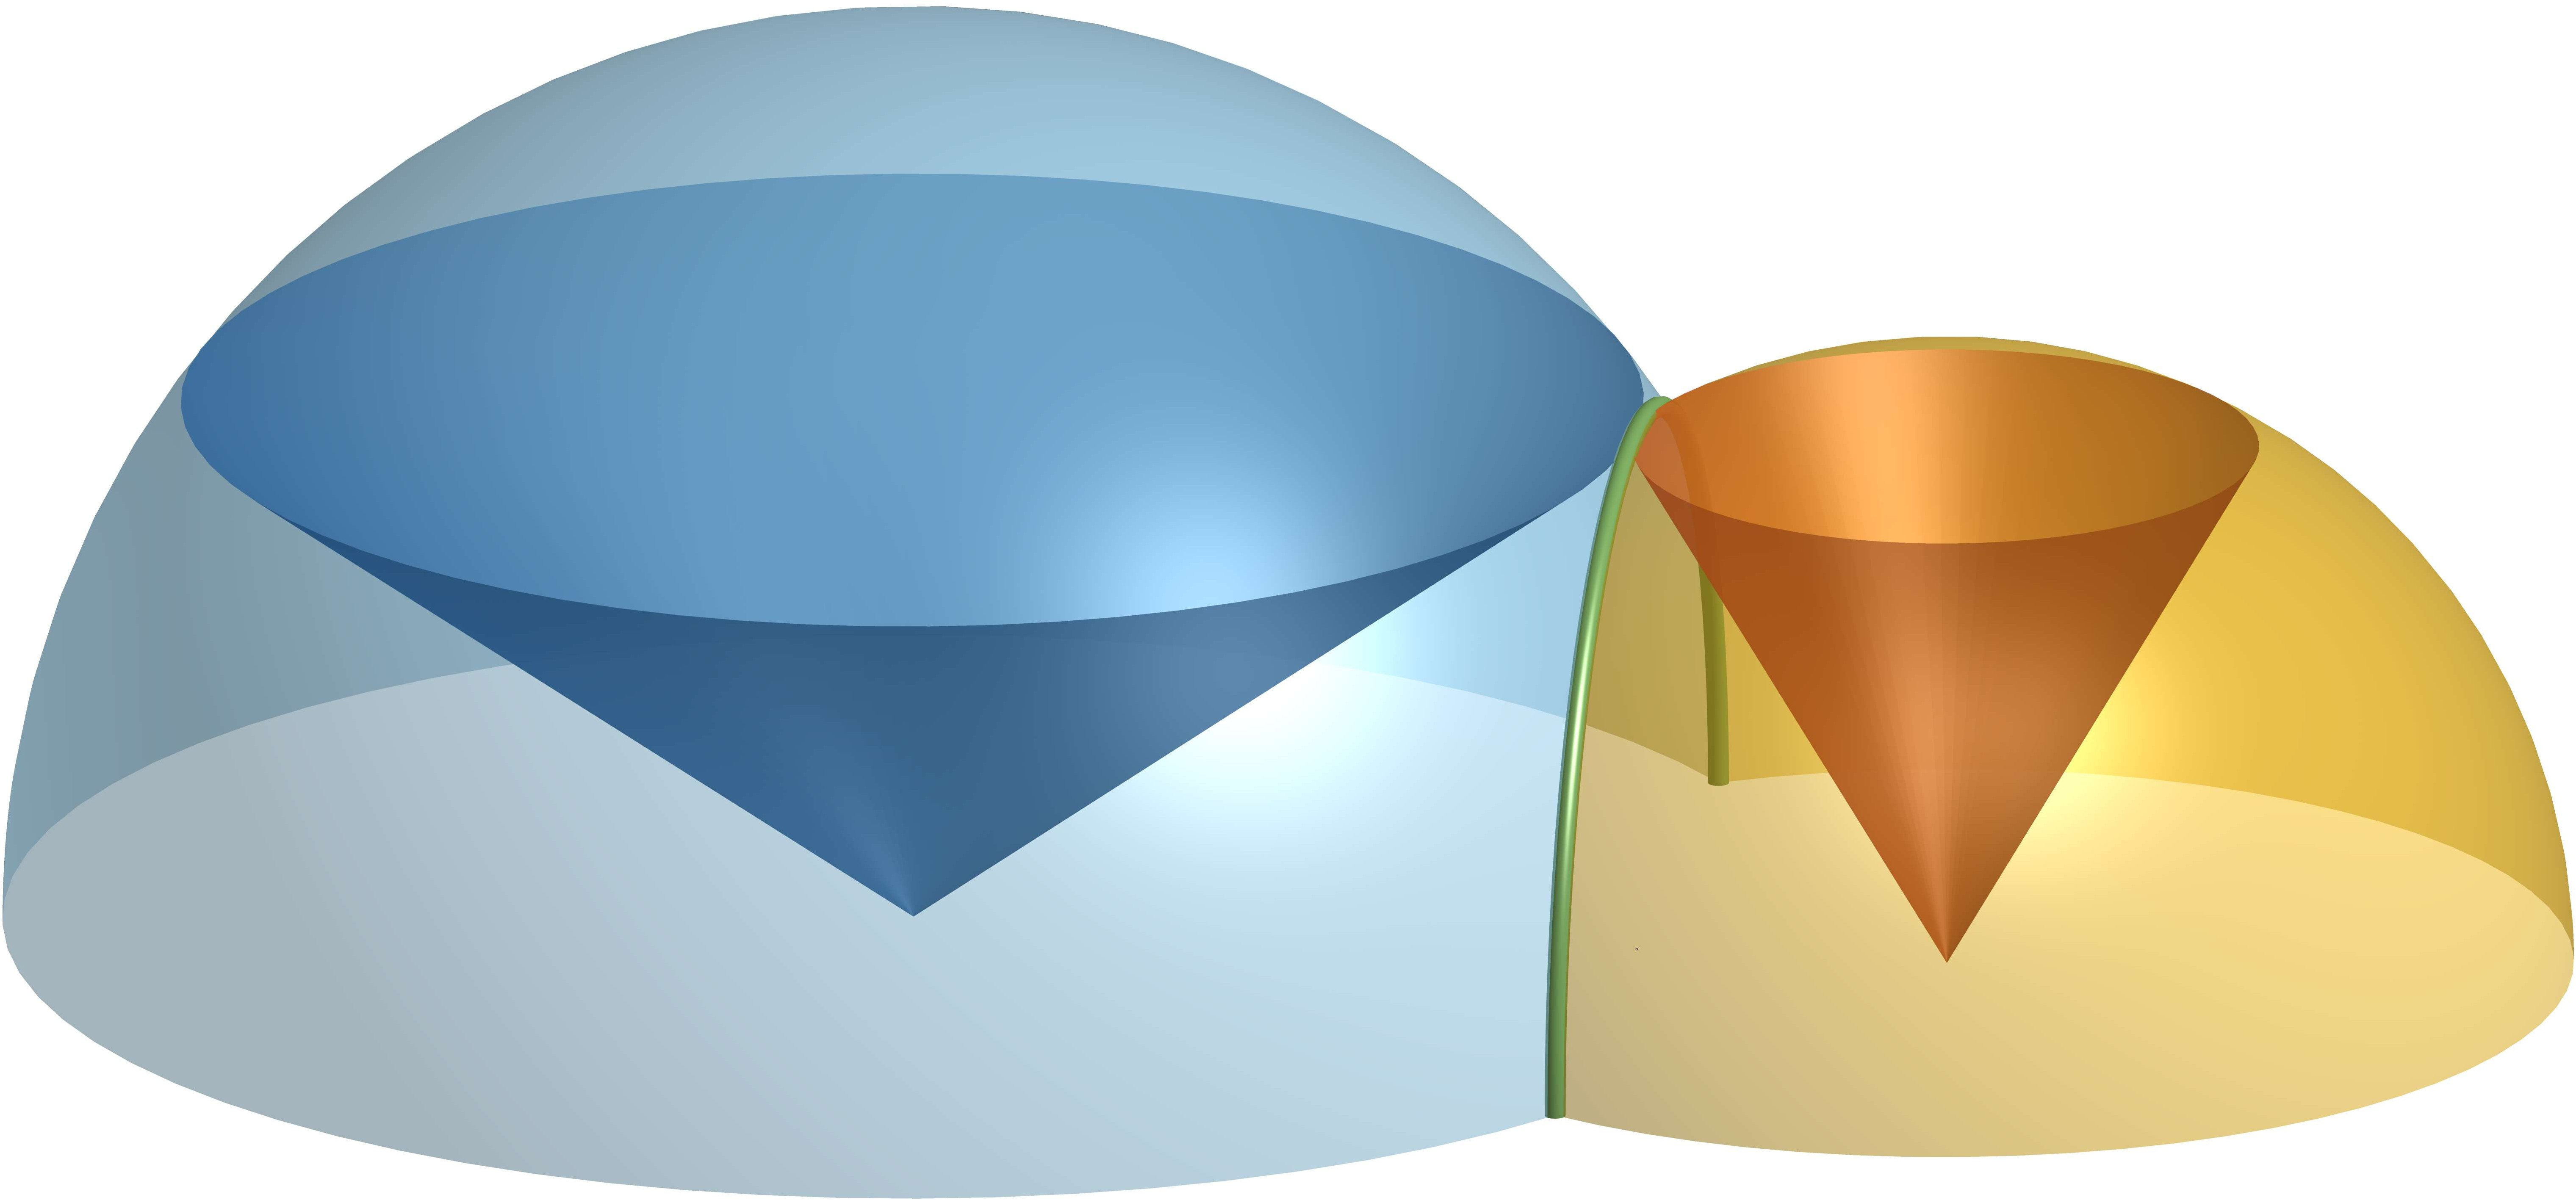
\includegraphics[max width=.75\textwidth]{gfx/diagrams/multisensor}
    \caption{3D rendering of a multi-sensor scenario: Two sensors are enough to
    single out a target's location, while a trilateration approach would require
    a third sensor to narrow down the location from the intersection circle
    (green) of the trilateration spheres (orange and blue) to the target location (purple dot).}
    \label{fig:multisensor}
\end{figure}

The method also helps when more than one target is visible and they need to be discerned from each other: while many trilateration spheres intersect in larger or smaller circles, the cone base edges touch (or, with added noise, are very close) only for the same target.

2D target location resolution is completely sufficient for mobile ground robots. Hence the rest of this thesis will focus on the side- and forward-facing 2D geometry described in \cref{geometry-for-the-general-case}.

\section{Doppler speed estimation}\label{doppler-speed-estimation}

In order to estimate the reprojection angle with \cref{eq:geometry_side_alpha}, the target Doppler speed $v_D$ must be measured. If the measurement is not precise, the reprojection angle \(\alpha\) will be imprecise and noisy. A map built with noisy observations will contain smeared-out targets or even false positive detections on the map.

With FMCW radar, a target's range and Doppler speed can be simultaneously registered. Especially at low speeds the speed resolution or accuracy may not be not very high with this method. Doppler speed can instead be estimated from a target's change in range over time. The development of the peak gradient algorithm that accomplishes this with subsample resolution is detailed in \cref{doppler-estimation-with-the-peak-gradient-algorithm}.

\section{Map building}\label{reprojection-method}

As soon as a target's range and angle are known, it can be mapped in relation
to the radar's position. The radar position can be assumed at the map's origin for the first measurement; however the radar's translation and rotation relative to this start position needs to be known for subsequent measurements. This can easily be achieved with proprioceptive sensors such as inertial measurement units (IMUs) and encoder odometry. To compensate odometry drift in longer scans position corrections from absolute position sources should be integrated. Such a source is usually available from a magnetometer for heading, from global navigation satellite system (GNSS) sensors (e.g. GPS), motion capture camera systems or other ground truth systems \cite{Godil2013}. It is also possible to run a slam algorithm or probabilistic localization like adaptive Monte Carlo localization (AMCL) for localization.

Building and updating of the map at a detected target location can either be in form of a binary target indicator, or with a probabilistic distribution. The latter can be taken from the target peak in the sensor's range profile.

The map can then be further processed with path planning algorithms such as Dijkstra, A*, D*, probabilistic road maps (PRM), and rapidly-exploring random trees (RRT) to allow intelligent path planning and obstacle avoidance for mobile robots \cite{Correll2016}.

\section{Limitations}\label{limitations}

The reprojection method has some inherent limitations. The most obvious one is that since target angles are calculated from radial target speed, all objects must not have a speed of their own, i.e. they must be static. This limitation however sounds more severe than it is in practice. On the one hand, robots often operate alone and without any other moving objects present, such as a vacuum robot cleaning the house while its owner is at work. On the other hand, if moving objects appear, such as a cat quickly escaping the vacuuming noise, they can be detected and tracked as soon as their radial speed exceeds the robot speed.

In 2D geometry, target echos must be limited to one plane and in the preceding explanation, this is assumed. If this is not the case, target elevation needs to be estimated in addition to target azimuth. With an antenna beam pattern that limits sensitivity to planar elevation, coplanarity of all targets can be assumed.

Another noteworthy issue is that real-world targets may not be adequately represented by a point target. However, especially if Doppler speed is estimated from peak gradient, any target visible in a range scan can only have one radial speed associated with it. If a long wall is visible over many range bins, the reprojection angle will be calculated from the speed of the peak point in the wall's echo. A map entry will be line-shaped with an angle corresponding to the point of strongest echo intensity, which is usually orthogonal to wall orientation, and with a length corresponding to detected peak width, which depends on the objects reflectivity at different incident angles. In effect, a wall will be built up on the map as the robot passes it, and the mapped wall thickness will be slightly influenced by how much of the wall reflects in a single range scan (usually a few centimeters, short solid red line in \cref{fig:wall}).

\begin{figure}[htbp]
    \centering
    \def\svgwidth{7.5cm}
    \input{gfx/diagrams/wall.pdf_tex}
    \caption{Walls reflect only at limited, material-dependent backscatter angles. They thus appear as point targets with a Doppler speed equal to the radar's motion component orthogonal to the wall.}
    \label{fig:wall}
\end{figure}

Lastly, without direct Doppler measurement, only one target can be detected at any range bin. This limitation does not strongly affect practical operation, because situations where several targets are at the same range for more than a few seconds are very rare or can be easily avoided. For example, both walls of a corridor can be detected if the radar is not moving exactly in the middle of the corridor.
